\section{Arquitectura del Sistema}

\subsection{Estructura General y Comunicación IoT}
El sistema se organiza en tres capas jerárquicas interconectadas mediante el protocolo MQTT, como se ilustra en la Figura~\ref{fig:diagrama_arquitectura}:
\begin{enumerate}[noitemsep]
    \item \textbf{Capa de Percepción (ESP32):} Adquisición de magnitudes físicas, control de salida digital y cliente MQTT (\texttt{PubSubClient}).
    \item \textbf{Capa de Transporte (Red local + Mosquitto):} Enlace inalámbrico Wi-Fi y servidor de mensajería MQTT (puerto 1883).
    \item \textbf{Capa de Aplicación (Node-RED):} Flujo de eventos y panel gráfico interactivo en Dashboard 2.0.
\end{enumerate}

\begin{figure}[H]
    \centering
    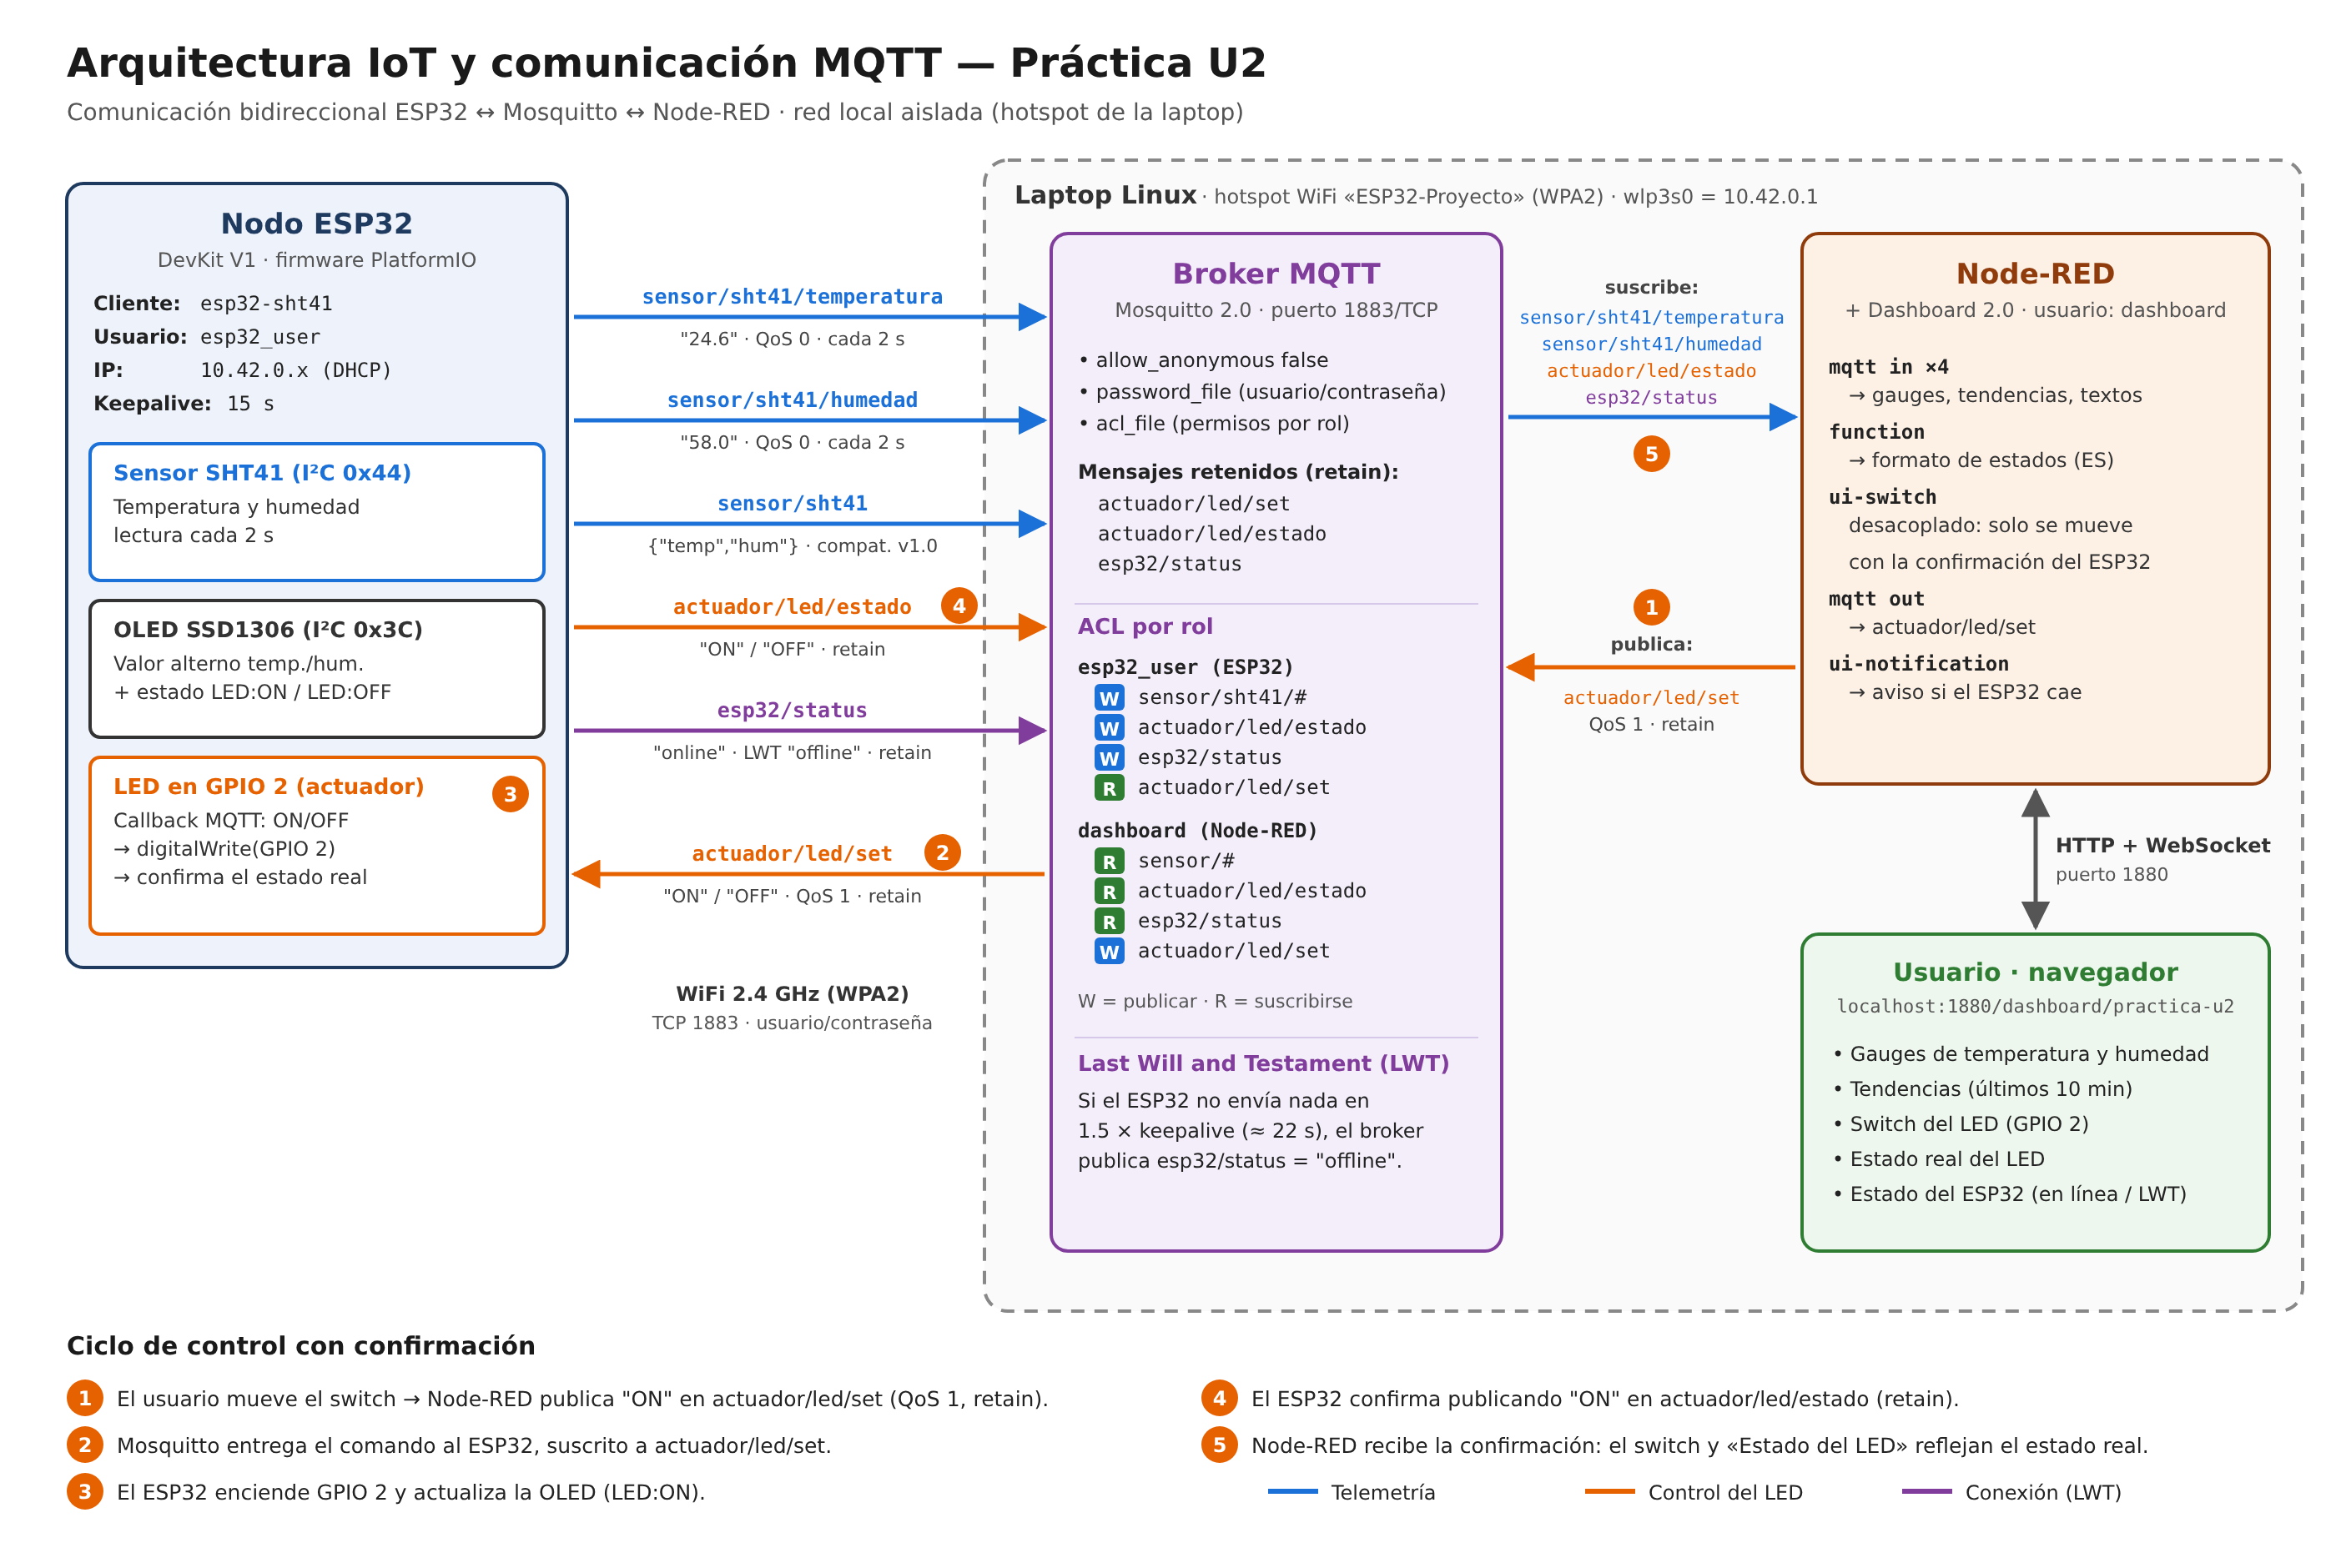
\includegraphics[width=0.96\textwidth]{imagenes/diagrama_arquitectura.png}
    \caption{Arquitectura general del sistema, red local y comunicación bidireccional MQTT.}
    \label{fig:diagrama_arquitectura}
\end{figure}

\subsection{Configuración de Red Local (Hotspot)}
\begin{itemize}[noitemsep]
    \item \practicaBadge \textbf{Enlace Wi-Fi:} La ESP32 se conecta como estación (\texttt{WIFI\_STA}) al punto de acceso local bajo cifrado WPA2.
    \item \proyectoBadge \textbf{Red Aislada de Laboratorio:} La laptop genera el punto de acceso mediante NetworkManager (\texttt{nmcli}), asignando una subred privada fija \texttt{10.42.0.0/24} con IP del broker en \texttt{10.42.0.1}. Esto aísla el tráfico de redes institucionales y asegura que el puerto 1883 no sufra bloqueos de cortafuegos externos.
\end{itemize}
